% TODO: Change font to helvetica
% double spacing

% latex template
\documentclass[12pt]{article}
\usepackage[utf8]{inputenc}
\usepackage[english]{babel}
\usepackage[margin=1in]{geometry}
\usepackage{caption} % figure captioning
\usepackage{amsmath} % equation tools
\usepackage{amssymb} % math symbols
\usepackage{mathtools} % math rendering improvements
%\usepackage{siunitx} % standard units
\usepackage{graphicx} % add images
%\usepackage{wrapfig} % position images
\usepackage{float} % position images pt.2
%\usepackage[makeroom]{cancel} % cross out text
%\usepackage[version=4]{mhchem} % chemical equations
%\usepackage{multicol} % multiple columns
%\usepackage{pgfplots} % built in plotter
%\pgfplotsset{width=10cm,compat=1.9} % plotter settings
\usepackage{hyperref} % table of contents links
\usepackage{indentfirst} % indent first paragraph after section

\hypersetup{
    colorlinks,
    citecolor=black,
    filecolor=black,
    linkcolor=black,
    urlcolor=black
}

\renewcommand{\baselinestretch}{1.5} % line spacing
\newcommand{\fline}{\par\noindent\rule{\textwidth}{0.1pt}} % horizontal line (wide)

\title{EE TITLE}
\author{Bryan Deng}
\date{}

\begin{document}

\maketitle
\newpage
\tableofcontents
\newpage

\section{Background Information}

\subsection{Machine Learning and its Applications}

Machine learning (ML) is a branch of artificial intelligence that uses large datasets and algorithms to mimic the way humans learn and improve accuracy over time \cite{what_is_ml_ibm}. Since its debut in 1952, it has been steadily gaining popularity for its abilities in recognizing patterns and continuous learning. Machine learning powers many of the applications we use on a daily basis, including chatbots, language translation tools, and social media feeds \cite{what_is_ml_mit}.

Where machine learning shines is in its ability to solve problems that would typically be either impossible for impractical for traditional algorithms. Furthermore, machine learning models are able to generalize these solutions and apply them to additional problems it has never encountered before.

In short, machine learning is a combination of computer science, statistics, and optimization. It uses knowledge from different fields to ``teach'' computers to complete tasks. As the model looks at more and more data, it starts to recognize patterns among it and optimizes itself.

\subsection{Decision Trees}

When most think about machine learning, the first thing that comes to mind are neural networks. Neural networks, which are abstractly complex yet powerful algorithms, only make up one subfield of machine learning itself, called \textit{deep learning}. However, there exist several other branches of machine learning, such as \textit{supervised learning}, the main focus of this paper. The most well known model within supervised learning has to be the decision tree. They are binary trees which employ a straightforward \textit{if-else} flow to classify data.

\begin{figure}[H]
    \centering
    \fbox{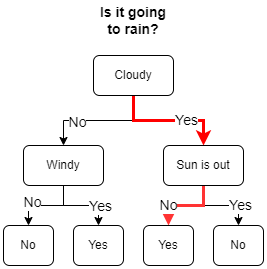
\includegraphics[scale=0.7]{figs/decision_tree.png}}
    \caption{Decision Tree Diagram}
    \label{fig:decisiontree}
\end{figure}

\hyperref[fig:decisiontree]{Figure 1} shows a simple decision tree to predict whether it will rain based on other weather conditions. Given a cloudy day with no sun, the model will predict that it will rain, as outlined by the red lines on the diagram. The anatomy of a decision tree consists of several parts \cite{dt_skl_doc}:

\begin{itemize}
    \item \textbf{Node}: cells that contain data. A tree is made of several nodes connected by edges.
    \begin{itemize}
        \item \textbf{Root node}: the single node at the very top of the tree.
        \item \textbf{Split node}: a split node splits into two other child nodes based on a feature and split value.
        \item \textbf{Leaf node}: a node at the end of a tree; it does not split into further nodes.
        \item \textbf{Child node}: the nodes that follow split nodes.
    \end{itemize}
    \item \textbf{Feature}: an individual characteristic of a dataset \cite{pattern_recognition_ml}, the $i$th feature is represented as $x_i$.
    \item \textbf{Split Value}: a value that classifies any data that the node encounters (e.g. $x_i \le2.7$)
\end{itemize}

The main computational problem with decision trees is how first construct, then optimize them. If we were to generate a random decision tree structure, it could potentially become very large and unnecessarily complex, taking up extra resources in computation. And if we were to simply assign each node a random feature and split value, it is very unlikely the model will perform well in predictions.

The approach used in vanilla decision trees is a greedy top-down algorithm that builds nodes, assigning it features and split values as it moves down the tree \cite{dt_induction}. Other well-established algorithms for constructing decision trees include random forests and gradient boosting. This paper aims to investigate a new decision tree construction and optimization algorithm by employing the genetic algorithm.

\subsection{Genetic Algorithm}

Taking a page straight out of Darwin's theory of evolution, genetic algorithms employ the principle of \textit{survival of the fittest}. It generates populations of algorithms or models that evolve and reproduce over time based on a set of criteria, improving on performance. Each \textit{individual} of the population is represented by a form of data structure. Each piece of data can be paralleled to a gene, which when all combined describes the behavior of the individual \cite{intro_to_ga}. The steps of the genetic algorithm are as follows:

\begin{itemize}
    \item \textbf{Initialization}: an initial population is generated with random genes using a set of preset hyperparameters.
    \item \textbf{Fitness evaluation}: a score given to each individual in the population based on how well it performs for the problem.
    \item \textbf{Selection}: a process to select the individuals that will carry forward or reproduce for the next generation, usually based on fitness.
    \item \textbf{Crossover}: a process to either sexually or asexually reproduce individuals for the next generation based on the previous generation.
    \item \textbf{Mutation}: randomly altering genes of an individual to maintain diversity and encourage further exploration of the solution space.
    \item \textbf{Termination}: a set of criterion to determine when reproduction for new generations should stop.
\end{itemize}

The species in real life which benefit the most from evolution are those that are able to maintain diversity. With diversity, they can overcome external problems like diseases or natural disasters. Similarly, the genetic algorithm puts a strong emphasis on diversity, so it can explore a large solution space and escape falling into a local minimum. Diversity is achieved with several stages of randomness introduced in each generation, in selection, crossover and mutation.

\section{Evolutionary Decision Tree}

An Evolutionary Decision Tree (EDT) uses a genetic algorithm to optimize decision trees. It aims to take the benefits from both vanilla decision trees and random forests, while adding a layer of optimization that increases its accuracy with training.

Similar to vanilla decision trees, an EDT is able to output a singular or small number of low complexity trees. The first of the two advantages of this output is that it makes the tree comprehensible by humans and easy to follow along. But more importantly, it avoids overfitting of the training dataset, a major downfall of overly complicated and large decision trees.

And similar to random forests, EDT's are able to harness random number generators to explore a larger solution space, thereby minimizing the chances of fitting into a local solution.

\subsection{Evolutionary Process}

The steps in constructing an EDT are built closely on the steps of the genetic algorithm. Each step has been modified or tweaked to support operations with binary trees.

\subsubsection{Initialization}

The EDT population is composed of $n$ random generated decision trees, where $n$ is the population size. A randomly generated tree starts with a root node. Each of its children is then either a split node or a leaf node, according to a probability $p$. This step is repeated until a maximum desired depth is reached, or until all branches end in leaf nodes \cite{faik_2020}.

\begin{itemize}
    \item If a node is a split node, it is randomly assigned a feature and split value.
    \item If a node is a leaf node, it is randomly assigned a label. Further restrictions are put in place to ensure that no branch in the tree can only lead to a single label.
\end{itemize}

\subsubsection{Fitness Evaluation}

The fitness for each individual in the population will be measured by the following formula \cite{faik_2020}:

\[F_i = c_1 \cdot a_i + c_2 \cdot f(d_i)\]

\begin{itemize}
    \item $F_i$ is the fitness of the $i$-th individual.
    \item $a_i$ is the accuracy of the $i$-th individual on the training data.
    \item $d_i$ is the depth of the $i$-th individual.
    \item $f(x)$ is a predetermined function.
    \item $c_1, c_2$ are predetermined constants.
\end{itemize}

\subsubsection{Selection}

The selection process will be a combination of two separate algorithms. The first of which will be tournament selection. A random set of $k$ individuals will be ranked by fitness, and the highest score will be able to move on to the crossover stage. This process is repeated twice, once for each parent in crossover. The random nature of this selection process ensures that diversity is maintained between generations, and that certain traits will not be entirely lost \cite{blickle_1997}.

The second selection process will be elitism. This is where the fittest individuals from the previous generation will be moved directly on to the current generation, without crossover. This is to ensure that the traits of the best individuals are not lost through generations.

A total of $t$ individuals will be moved onto the next generation through elitism. The remaining $n - t$ spots will be filled through tournament selection and crossover.

\subsubsection{Crossover}

For crossover, two parent trees will produce two child trees in order to maintain the population count. The first child will originally be a direct copy of the first parent. A random node is then selected from each parent. The node from the first parent, and its entire subtree, will be replaced by the node from the second parent and its subtree.

% TODO: add diagram for crossover

\subsubsection{Mutation}

If a tree is chosen for mutation, it will have one of its values traits randomly chosen and randomly altered. If the node selected is a split node, its feature and split value will be altered. Otherwise, if the node selected is a leaf node, it will have its label altered.

\subsubsection{Termination}

There are two conditions for termination. The first of which is when the number of generations has reached a predetermined $n$. The other condition is when the average fitness does not improve by a predetermined threshold for $x$ generations. Which ever condition comes first is when the EDT will terminate.

\section{Experimental Methodology}

The goal of this investigation is to compare an EDT to other classification algorithms including a vanilla decision tree, random forest classifier, and a multilayer perceptron.

\subsection{Independent Variables}

Three datasets of varying sizes will be used.

\begin{center}
    \begin{tabular}{|c|c|c|c|}
        \hline
        Dataset & Features & Labels & Instances \\
        \hline \hline
        \href{https://archive-beta.ics.uci.edu/ml/datasets/breast+cancer}{Breast Cancer} & $10$ & $2$ & $286$ \\
        \hline
        \href{https://archive-beta.ics.uci.edu/ml/datasets/mushroom}{Mushroom} & $23$ & $2$ & $8124$ \\
        \hline
        \href{https://archive-beta.ics.uci.edu/ml/datasets/adult}{Adult} & $15$ & $2$ & $48842$ \\
        \hline
    \end{tabular}
\end{center}

\subsection{Dependent Variables}

\section{Data Analysis}

\section{Error Analysis}

\section{Conclusion}

\section{Appendix}

\bibliographystyle{plain}
\bibliography{refs}

\end{document}

